\chapter{Method Implementation And Results}

In this chapter the tools used, the software infrastructure and method implementation and the results collected during the analysis are reviewed.

A DDPG Agent\footnote{An agent whose actions are taken by a neural network trained with the reinforcement learning algorithm DDPG} was trained to drive in an urban environment. Checkpoints of the network's state during the training were recorded for the purpose of comparison. These checkpoints of the network were then tested with and without a simple safety-monitor in order to provide a new point of view to study AV's behaviours.

\section{Tools and software}

\subsection{Carla Simulator}

In order to have a realistic environment, with accurate physics simulation and data sensors, the open-source simulator CARLA\cite{carla}, developed by researchers at the University of Barcelona, was used. This simulator was developed with the purpose of offering an environment where AI agents can be trained to drive, with high control of the simulation parameters and the simulation of realistic sensor, which can be tuned to increase or decrease data quality, or to inject faults.\newline
CARLA is developed with a client-server architecture in mind. The \textsl{server} is basically a game, developed with \textsl{Unreal Engine 4} in C++. C++ performances are with no doubt essential to the functionality of the server: not only the environment must be simulated (including movements of pedestrians/vehicles, weather simulation\dots), but also all the data needed from the sensors attached to the system.\newline


\begin{figure}[h!]
	
\includegraphics[width=\textwidth]{img/carla.jpg}
	\caption{CARLA logo at carla.org}
\end{figure}

CARLA is currently at version 0.9.7 and huge improvements are done at every release, gaining more attention from the experts for its realism. Unfortunately, when this study started, CARLA 0.9 was recently released and the tools needed for our work couldn't be found online. Thanks to the quantity of work done for the last \textit{stable} version of CARLA, 0.8.4 was used at first.\newline
Versions prior to 0.9 have some limitations on the control one has of the simulations parameters and on the data collectable from it. This doesn't impede our study, but of course limited in some way the informations on the environment and system. Some of these problems are still present in later versions of the simulator, but most of them were solved in the transition from 0.8 to 0.9.\newline\newline
One of the main problems found was with the coordinate systems. Before version 0.9, developers were using UE4's default coordinates system which is left-handed, while the standard is considered to be right-handed. This looks like not a big deal since things could be easily solved by applying a transformation matrix. However, due to performance issues (a Python client should do the real-time processing of \textsl{loads} of data at each timestep, resulting in considerable slowdowns as a result of all the processes running at the same time), it was decided to stick with the developers' decision and convert the data during analysis phase.

Unfortunately, this version of CARLA has only 4 sensors available, which were all used during the experiments. They can be easily accessed via the Python APIs provided:

\begin{itemize}
	\item Cameras
	\begin{itemize}
		\item The \textsl{scene final} camera provides a view of the scene (just like a regular camera)
		\item The \textsl{depth map} camera assigns RGB values to objects to perceive \textsl{depth} of the environment
		\item A \textsl{semantic segmentation} is used to classify different objects in the view by displaying them in different colors, according to the object's class
	\end{itemize}
	\item Ray-cast based Lidar
	\begin{itemize}
		\item Light Detection and Ranging is use to sense the environment and measures distance from objects by illunating the target with laser beams and measuring the time reflected light needs to "go back" to the sensor
	\end{itemize}
\end{itemize}

The three cameras were used during the training phase of the network. Three \textsl{scene final} cameras are attached to the car to actually \textsl{see} the environment (one on the front and one per side). The \textsl{depth map} camera allows the car to get a colormap of the distances from objects in the scenario.
The \textsl{semantic segmentation} provides image classification features by querying the server for ground-truth values. This is with no doubt a semplification of a real system, where the most powerful image-classification softwares are essentially other neural networks trained separately. At the same time a misclassification can be considered as an error of the control system: if the safety monitor detects the possible hazard it will not "correct" the misclassification but it must react fast and safely to avoid the possible consequences of it, therefore this simplification won't have an impact on the overall method.\newline

A ray-cast based Lidar is the only other sensor available for this version of CARLA. Parameters of this sensor can be easily tuned to simulate real lidars such as the \textsl{Velodyne LiDAR} or to simulate faults such as low data quality, noisy data or data loss\dots This data are generated using the \textsl{Point Cloud}\cite{pointcloud} format

In the simulations, due to the high hardware resources requirements to simulate a real LiDAR, a slightly modified version of the \textsl{Velodyne64 LiDAR} is implemented with the following parameters:

\begin{itemize}
	\item Channels = 64
	\begin{itemize}
		\item The number of laser beams used by the system. These lasers are distributed over the vertical axis. The more the lasers are, the more accurate will be the scannings
	\end{itemize}
	\item Range = 75m
	\begin{itemize}
		\item Lasers' range in meters
	\end{itemize}
	\item Rotation Frequency = 15 Hz
	\begin{itemize}
		\item This parameters define the rotation frequency (in Hz) of the scanning beams.
	\end{itemize}
	\item Points Per Second = 1.000.000
	\begin{itemize}
		\item The actual number of points generated each frame by the sensor
	\end{itemize}
	\item Vertical FOV bounds (height = 24m, low = -2m. Distances are relative to the position of the sensor)
	\begin{itemize}
		\item Maximum and minimum height of the scannings
	\end{itemize}
\end{itemize}

The simulator provides Python APIs not only to modify sensors, but also to have a great control on what is being simulated, such as seeds definition for the spawning points and the behaviours of pedestrians and vehicles, and on the state of \textsl{"actors"} in the scene such as their position, their speed\dots. All these data are directly provided by the simulator with ground-truth values. These kind of measurements can be simulation-related, such as the simulation time-step, or the FPS. Actors-related measurements include for example vehicles' speed, intensity of collisions (if any) and the 3D acceleration vector.\newline

While this tool was being tested a problem was found with the LiDAR sensor data that is still not resolved.\cite{lidarbug} 
The bug resulted in the vehicles' bounding boxes to be distorted when moving, providing very poor data.
After some research an improved version of the simulator was found, where the bounding boxes for each vehicle were redefined to provide accurate data.\cite{carlapro} As of today, developers are working on this issue but it is still unresolved without manual intervention on the source code.


\subsection{Controller Implementation}

The main component needed for the Controller implementation is the neural network that will be in charge of deciding the action to perform to drive the car. We looked for a framework with the following characteristics

\begin{itemize}
	\item[1] Training code must be available
	\item[2] No critical issues in the codebase
	\item[3] Provide an environment to interface the network with CARLA
	\item[4] Provide a default training strategy
\end{itemize}

After analyzing all the machine-learning related projects for CARLA, we chose the reinforcement-learning framework \textsl{Coach}, developed by \textsl{Intel AI Lab}.\cite{coach}

This framework satisfies all the requirements listed above: it is distributed as an \textsl{editable Python package}. The development team behind this project assure us the quality of the product. Moreover, several presets are available as a starting point. Two of these presets offer an interface to the CARLA simulator, as well as a default training strategy, which is exactly what we required.

These presets implement the \textsl{Deep Deterministic Policy Gradient} algorithm, proposed in 2015.\cite{ddpg} This algorithm proved to perform well in tasks such as car driving, as shown in the original paper, and it's specifically adapted to perform in environments with continuos action space, such as the one we are considering.

\begin{itemize}
	\item[P1)] The first preset uses a single, front camera to perceive the environment, and the other data augmentation cameras provided by CARLA. The agent resulting from using this preset will likely not have any sense of depth created by the regular camera and will rely solely on the depth camera
	\item[P2)] This preset uses all the cameras available in CARLA and have a much more interesting architecture since the car is equipped with three regular cameras (Front, Left, Right) and all the data augmentation cameras available in CARLA, listed in the previous section
\end{itemize}

The usage of the data augmentation cameras (depth and semantic segmentation) allows us to ignore objects misclassifications (e.g. labeling a pedestrian as a light pole) as well as some other easinesses such as computing distances from objects. As pointed in the previous section, this is indeed a simplification of a real architecture, where object detection modules are neural networks themselves, that must be trained in advance and tested separately. However, again, a misclassification will probably cause the Controller to behave in unexpected manners that the Safety Monitor must be able to detect and possibly correct.

Unfortunately, the first preset suffers from an issue that causes the car to stop throttling, while being positively rewarded\cite{coachIssue}. It would have been interesting to test this preset as well, to understand what's the impact on the effectiveness of the Safety Monitor with respect to the quantity of data available to the network.\newline

It's important to notice that our goal \textsl{is not} to build the \textsl{"perfect"} agent, nor the perfect autonomous cars. The codebase was studied but, due to reasons of time, we could not inspect all the details of the provided implementation. This framework was used as an example to demonstrate the concepts described in this work.


\subsection{Safety-Monitor Implementation}

In order to start the experimental activity, we needed a software capable of processing LiDAR data to map the environment and sense the obstacle. Moreover, this software needs to be \textsl{real-time} and capable of interacting with CARLA. The latter is obvious: whenever an alert is raised, the \textsl{"brake"} command must be sent to the CARLA server. The first required some reasoning: one could think to record the LiDAR data in advance and then run the simulations feeding the Monitor with these data. Unfortunately this approach can not work: this comes from the fact that we are not only interested in having a 100\% prediction accuracy, but also in the \textsl{goodness} of the safety-measure adopted by the Monitor. The same measurement in two different simulations could give \textsl{slightly} different results, that could cause the Monitor to behave in a completely different way than the way it could have behaved using the \textsl{real time} data produced during the simulation. If the accuracy of measurements is strictly dependent on the simulator used for the experiments (CARLA is improving at every release on this side), we could not ignore the effects that a brake can have on a single run.

In order to develop a decent Safety-Monitor, a research on the best, \textsl{"not-neural-network"} techniques was conducted, as well as a research on the open-source instruments available. The choice fell on the \textsl{Point Cloud Library}\cite{pcl}, an open-source library specifically dedicated to the processing of Point Cloud data, developed using C++ to achieve great performances when processing huge amount of data.
This library was first released in 2011\cite{pclwiki} and it's been improved at every release, also thanks to the big community testing and debugging the new features.

This library offers a multitude of functions that implements the most known techniques for Point Cloud processing. The steps to follow in order to develop an object-detection module are the following:

\begin{itemize}
	\item[1)] Downsampling
	\begin{itemize}
		\item[$\rightarrow$] The data generated by a single scan can contain more hundreds of thousands records, with possibly a lot of redundancy and noise. A downsample is usually necessary as a preliminary step to discard all the \textsl{"useless"} data. After some reasoning, the Voxel Grid Filter was chosen for this step
	\end{itemize}
\end{itemize}

\begin{itemize}
	\item[2)] Ground Segmentation
	\begin{itemize}
		\item[$\rightarrow$] After the downsampling (if needed), the first mandatory step is to filter the data that are useless for the purpose of object detection, such as points relative to the ground. These point must be filtered in order to separate the ground from the objects we want to detect.
		In our implementation this is done using the RANSAC\footnote{Random Sample Consensus} algorithm\cite{ransac}, a technique to separate \textsl{"inliers"} (i.e. data whose distribution is characterized by the model's parameters) from \textsl{"outliers"} (i.e. data that don't have a representation in the chosen model)
	\end{itemize}
\end{itemize}

\begin{itemize}
	\item[3)] Clustering
	\begin{itemize}
		\item[$\rightarrow$] This final step is required to effectively identify what is an object in the scene, and what data points are relative to the same object. This can be done using clustering algorithms based on the distance among points. We chose the Euclidean Clustering Algorithm, a range search algorithm based on the euclidean distance between points, with the assumption that \textsl{very dense} points represent the same object
	\end{itemize}
\end{itemize}

\begin{itemize}
	\item[4)] Object Tracking and Avoidance
	\begin{itemize}
		\item[$\rightarrow$] Objects detected in the first three steps must be tracked over time in order to recognize if two objects observed in two consecutive steps, are actually the \textsl{same} object, usually using physical models to predict their behaviour over time, such as the Kalman Filter, and combine this model with a failure-prevention routine
	\end{itemize}
\end{itemize}

Unfortunately, implementing a Kalman Filter for such a complex model would have been too much time-consuming, alting our study. Therefore we simplified the object-detection and the failure-prevention routine in this way:

\begin{itemize}
	\item Only data \textsl{in front of} the car are recorded. This is a huge semplification of the model, as the Monitor now can only detect obstacles ahead of the car. However, this will for sure have an impact on the effectiveness of the Safety Monitor, but the concepts explained in the previous section still holds
	\item The failure-prevention routine implemented takes inspiration from the Responsibility-Sensitive Safety model proposed by Mobileye, an Intel company.\cite{rss}
	If an object is detected, its speed relative to the system is computed. If the distance travelled by the system in 1 second  plus the braking distance is greater than the distance travelled by the object plus the distance between the system and the object, a safety brake is applied.
\end{itemize}

Since the Safety-Monitor is developed in C++, both for taking advantage of the Point Cloud Library and due to performance reasons, an infrastructure to exchange data with CARLA was developed.

The software is composed of a C++ server that receives LiDAR Point Clouds from the CARLA client. This data are processed as in the steps above (with the semplification described) and, if needed, an alert is sent back to the client. If the message received by the Monitor is an alert, the actions of the Controller are ignored and a brake is performed.

The object detection module is inspired by an open-source project developed by Engin Bozkurt\cite{LOD}. The codebase was deeply modified to adapt the detection algorithm parameters to fit our needs and to interact with CARLA.

We are conscious that this Monitor will likely not achieve "state of art" performances and it's likely to produce a lot of \textsl{false positives}. This aspect may have some consequences on the traning efficacy, but the concepts explained in this work still holds.

\section{Experimental Activity}

In this section is described how the methodology developed in the previous chapter was implemented, and the technical problems found during the implementation.

The Controller was trained in an urban environment, with the default strategy provided by \textsl{Coach} in order to generate four checkpoints to be subsequently tested.

Scenarios were generated using the 152 spawn points\footnote{Coordinates in the map in which the car will start its ride.} provided by Carla.
For each spawn point, a default setting and three variations of it were generated:

\begin{itemize}
	\item[h0)] \textsl{Default Setting}: the map is generated using the \textsl{same} conditions in which the Controller was trained, with 30 pedestrians and 15 cars
	\item[h1)] \textsl{Pedestrians Setting}: the map is generated increasing the number of pedestrians from 30 to 60
	\item[h2)] \textsl{Vehicles Setting}: the map is generated increasing the number of vehicles in the environment from 15 to 30
	\item[h3]) \textsl{Pedestrians and Vehicles Setting}: the map is generated merging $h1$ and $h2$, resulting in an environment with 60 pedestrians and 30 vehicles
\end{itemize}
	
For repeatibility, and consistency across the variations, 152 couples of unique seeds\footnote{These seeds are used in the generation of pedestrians and vehicles} were generated, each of them was associated to a starting point. This allows to use the same seed, for the same starting point, using different variations.

To enrich the informations about the System's overall performances, the car is also given a \textsl{Destination Goal} to reach, which is also recorded for repeatibility. If the Goal is reached, the success is recorded and the System is given a new destination to reach.\newline

In general, it may require a huge amount of time for a crash to happen. For this reason, in order to demonstrate the concepts explained in this work, it was defined a maximum running time of 15 minutes, after which the System's task is considered succeeded.

In the first phase of the analysis, four checkpoints generated were tested according to the methodology described in section 3.
Since the \textsl{Coach} project is open-source, the codebase was freely available. This allowed us to use \textsl{software probes} to monitor the Controller's activity.
The source code was modified adding some instructions to write all the needed data into different file for each run:

\begin{itemize}
	\item The starting point and seeds of the Scenario
	\item Actions taken by the Controller
	\item If there is a collision, with what
	\item If a goal is reached, record it and the new goal coordinates
\end{itemize}

Modifying the source code may in general result in a worsening of the overall performances, and the accuracy of results. Fortunately, the CARLA simulator provides an option to run the simulations at a \textsl{fixed-time step}. This was set at its minimum: 10 FPS\footnote{Frames Per Second}, to assure that all the data received from the server are \textsl{timely} and \textsl{correct}. This also serves as a mean for \textsl{repeatibility} of tests: a \textsl{variable time-step} may introduce randomness in data since we have no control over it.

The first training phase and the Controller testing required circa 1 month and a half to be performed.\newline

The second step was to test the effectiveness of the Safety-Monitor for each checkpoint.

The source code was once again modified to create two separate, concurrent processes: one takes LiDAR data from the CARLA server and sends them to the Safety-Monitor server; the other waits for the response of the Safety-Monitor to check whether a brake is needed.

The LiDAR data are generated by the CARLA server at each frame. The workload for data generation relies solely on the CPU, resulting in very much slower execution times. Unfortunately, CARLA suffers from a bug which causes data to be inaccurate, if FPSs are lower than 10. This required a powerful machine to guarantee the lower bound of 10 FPS.
The source code was once again modified to insert software probes in the codebase to gather informations about alarms raised by the monitor.

Runs recorded in the first step are now repeated observing the Safety-Monitor's behaviour. All the alerts raised during the run are considered \textsl{false positive}. The emergency brake is enabled 2 seconds before the collision, to estimate the amount of \textsl{true positives}.

This approach, allows us to estimate the goodness of the Safety-Monitor in its operational environment.\newline

After the first phase is concluded, data gathered are processed to compute the measures listed in the previous Chapter:

\begin{itemize}
	\item \textsl{Controller's Checkpoints}:
	\begin{itemize}
		\item[-] Mean Distance Between Failures
		\item[-] Mean Time Between Failures
		\item[-] Failure Rate
		\item[-] Reliability
	\end{itemize}
	\item \textsl{Safety-Monitor}:
	\begin{itemize}
		\item[-] Confusion Matrix of predictions
		\item[-] True/False Positives/Negatives Rates
		\item[-] Accuracy
		\item[-] Precision
		\item[-] Matthew's Correlation Coefficient
		\item[-] False Positives per Meter
	\end{itemize}
\end{itemize}

At this point, training is resumed from the last checkpoints using the strategies described before, and the measurement process is repeated identically.

Some of the strategies defined requires the training to be done \textsl{with} the Safety-Monitor, resulting in very low execution times. This phase took approximately 3 months because of the heavy computation load needed to generated LiDAR data, after which the training was stopped.

The numerical results collected can be compared to check if the network is learning properly and how the Safety-Monitor's effectiveness changes when the network improves.

Data collected were processed using \textsl{Python} scripts, to aggregate data in order to produce metrics of the \textsl{overall} performances of the Controller and the Safty-Monitor.
Data aggregation is fundamental for this kind of activity. At the same time, due to the complex nature of these systems and the fact that many hazardous events are \textsl{rare events}, it is \textsl{necessary} to study specific runs individually and to separately compare their performances before aggregating data as well (e.g. compare performances for the same Controller in each difficulty level).

In the next section we present collected results mostly in aggregated form, due to the huge amount of data collected. However, there are considerations on \textsl{"raw"} data that can not be shown in this work, but are attached separately for examination.

\section{Results}

\subsection{Phase 1 - Controller Testing}

The data collected are saved in separate files for each run and processed using Python scripts, computing the measures listed in Chapter 3.

The measures collected are compared to check the goodness of the Controller and changes in the effectiveness of the Safety-Monitor over the neural network's checkpoints.

Since the Checkpoints were tested in the \textsl{same} scenarios, the distances travelled for each scenario were plotted to check if meters travelled are increasing and if there are scenarios somehow \textsl{"favorable"} or extremely \textsl{"hard"} for the system. This first step allows testers to filter between critical scenarios and easy scenarios. Ideally, given a Scenario $x$, if the distance travelled by the Controller in $x$ is lower than the average distance travelled in all the checkpoints, there may be two cases:

\begin{itemize}
	\item[1)] In the case that the Controller always travels the same distance in all the checkpoints before crashing, there may be a hazard that the Controller has not learned to handle
	\item[2)] In the case the distance travelled fluctuates in a certain (small) interval, the happening of a crash may depend from the inital conditions
\end{itemize}

Regardless of the case, with this approach it's easy to see which scenarios make the Controller crash soon, and they can be examined individually with more attention.

It is important to keep in mind that if a trend is observed when testing different Checkpoints, e.g. a scenario in which the Controller \textsl{always} performs extremely good or extremely bad, an analysis of the specific case is needed, in both of the cases.

The reason is obvious for "bad" runs, for the reason listed above. It may seem counter-intuitive, but repeated "good" runs in the same scenario requires particular attention. An analysis of the correlation between performances and initial conditions is mandatory, and it may be demonstrated or confuted with this approach. A more complex case is when the System finds a \textsl{"lucky pattern"}, e.g. a run in which the car just follows the same pattern without finding any car on the road.\newline

Looking at charts of distances travelled in each scenario for Checkpoint 1 and 4 at \textsl{standard difficulty} below, it's obvious that the order of magnitude is quite different between the two checkpoints (C1 never travels more then 400 meters, while C4 has several runs longer than 1 km) and in a couple scenarios it has been reached the maximum length defined for these experiments.
Another very interesting fact observed with this approach, is that the lower bound on distance travelled doesn't change for $C2\dots 4$ and it's stuck at 22 meters in \textsl{all} the difficulties. A deeper analysis on travelled distances and running times shows that there are runs in which the Controller doesn't make any progress, as an indicator that the event causing a crash may be of a particular kind, which is hard for the Controller to handle. Results of this kind are with no doubt interesting in understanding if the shortest runs have some environmental conditions in common, which may cause the Controller to perform badly.

\begin{minipage}[c]{\textwidth}
	\includegraphics[width=\textwidth]{simulations/gen1/standard/distance-travelled-figure.pdf}
	\captionof{figure}{Meters travelled by Controller C1 (first Checkpoint) in each scenario at standard difficulty}

	\includegraphics[width=\textwidth]{simulations/gen4/standard/distance-travelled-figure.pdf}
	\captionof{figure}{Meters travelled by Controller C4 (fourth Checkpoint) in each scenario at standard difficulty}
\end{minipage}

The use of a \textsl{fixed time-step} when running the simulations, i.e. the simulation time elapsed between two steps of the simulation is fixed and known, gives us knowled of the interval of time between two consecutive actions: observing how many actions the Controller has taken it's possible to compute the \textsl{true} total time of a single run.

In this way, we are able to easily approximate the \textsl{Reliability Function} for each Checkpoint, based on the average MTTF in each level of difficulty.

\begin{figure}[h!]
	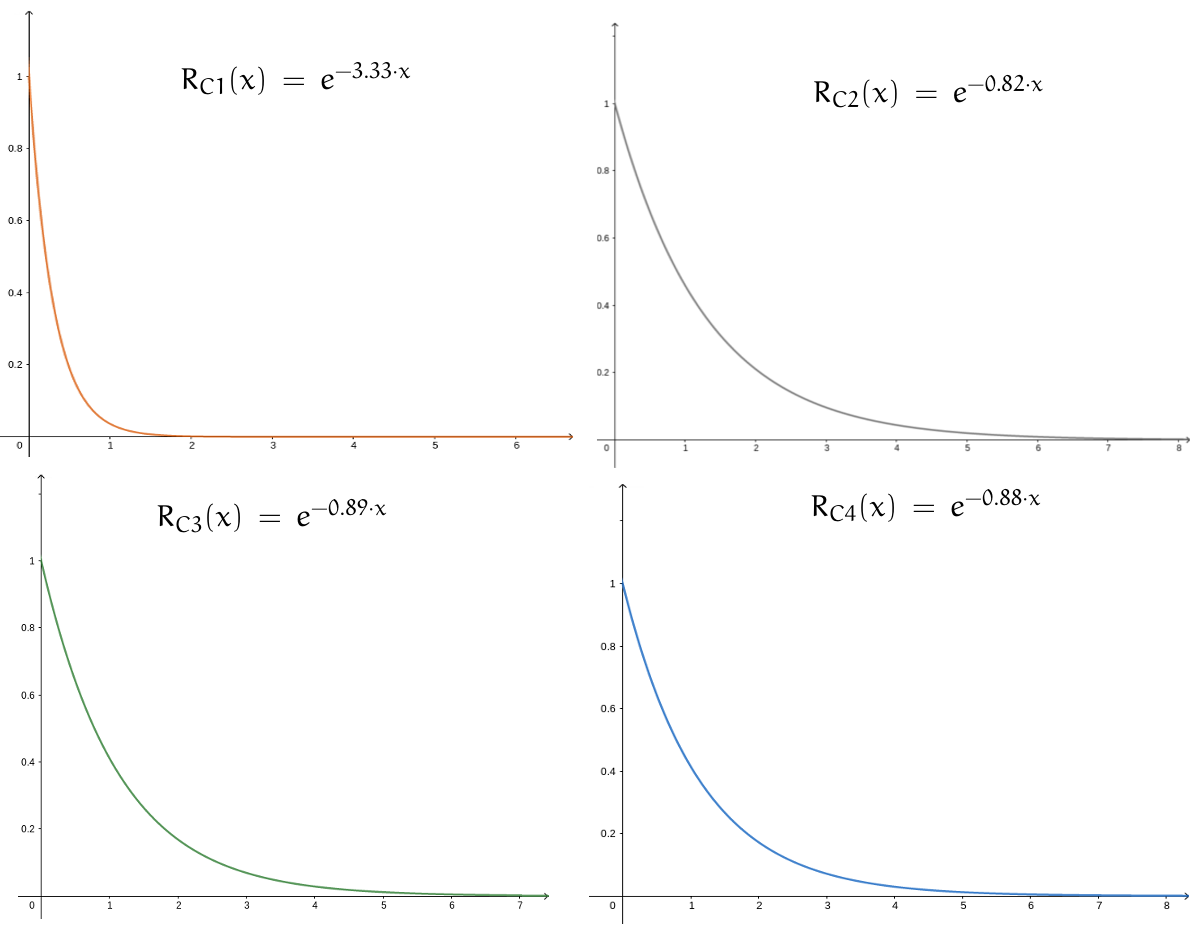
\includegraphics[width=\textwidth]{img/reliability-comparison.png}
	\caption{Graphics that shows the probability $y$ of the system being operational, after $x$ minutes of operation}
\end{figure}

As we expected, the MTTF of the first checkpoint is very low (20 seconds) and increases over Checkpoints. Surprisingly, the second Checkpoint seems to have better performances (higher MTTF) than Checkpoints 3 and 4. However, analyzing a subset of the runs in which the second Checkpoint achieved very good performances in terms of time to failure and distance travelled, it can be seen that its driving is way more dangerous than the other two, resulting in a bad driving style in which most of the times the car avoided a crash by steering at the very last moment. As another indicator of the fact that C2 is not really better than C3 and C4 is that it reached \textsl{Goals Destinations} fewer times than C3/C4, as another evidence that the \textsl{apparent} higher safety is likely to be a result of \textsl{"lucky patterns"} in the sense defined above (Goals reached charts are shown in \textsl{Section 3}).

Fortunately, as we will show with the results collected in phase 3, the Controller managed to overcome this problem.\newline

The same behaviour is observed for distances travelled by each Checkpoint: longer runs are actually runs in which the car travels more meters. This assure us that the system is not \textsl{"cheating"}: a longer execution time may come from the car not moving at all. Computing the average distance travelled by each Checkpoint in each difficulty level, allows us to approximate the Reliability Function in terms of kilometers travelled before crashing.

Moreover, the observed progresses in the \textsl{mean distance to failure} seems to follow the progresses of the \textsl{mean time to failure}, which is another assurance of the correspondence between the two metrics.

\begin{figure}[h!]
	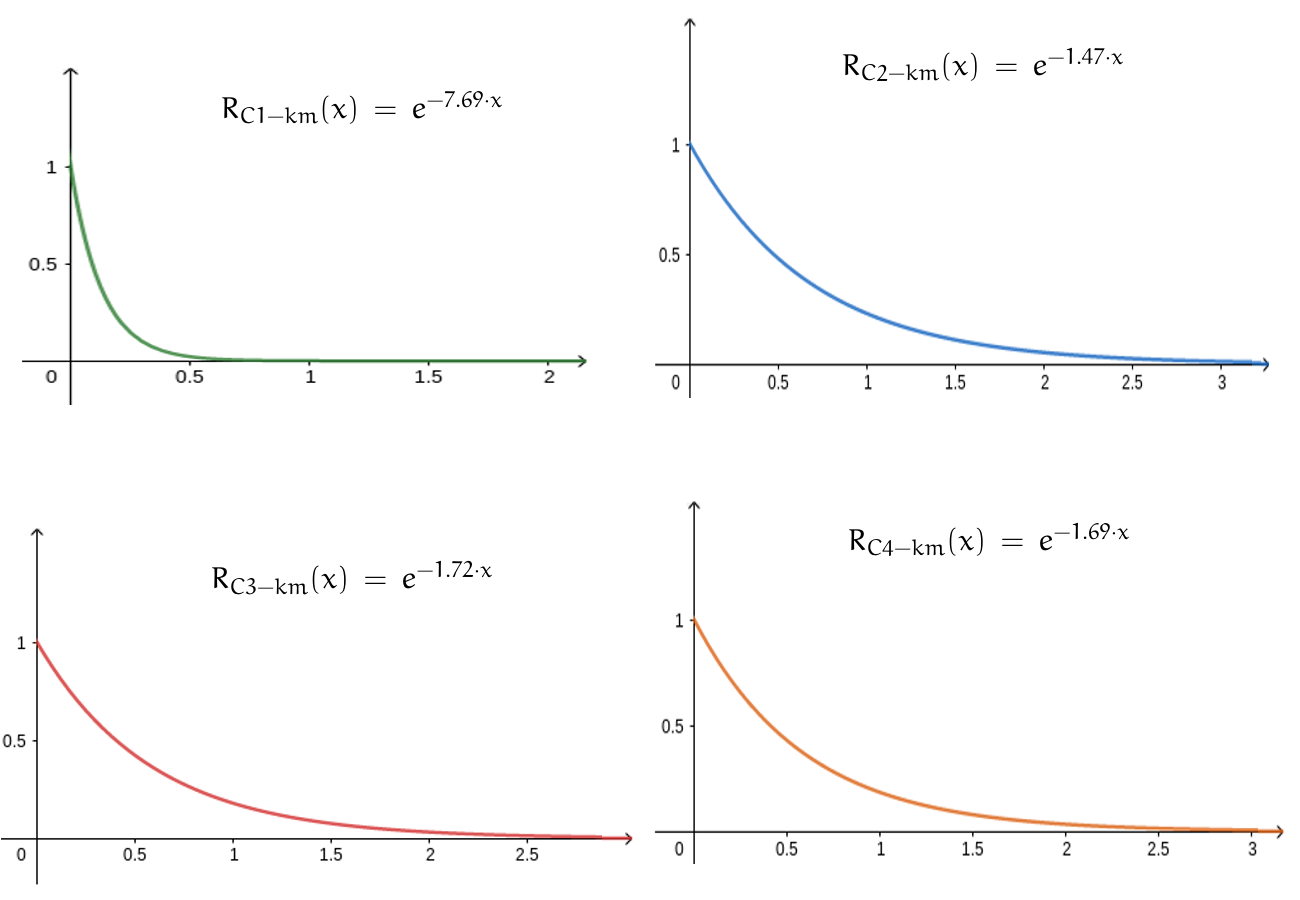
\includegraphics[width=\textwidth]{img/reliability-meters-comparison.png}
	\caption{Graphics that shows the probability $y$ of the system being operational, after $x$ kilometers}
\end{figure}

As another mean to analyze the Controller's behaviour over Checkpoints, since CARLA provides means to record the kind of object with which a collision occured, rates of kind of object collided with respect to total collisions are computed for each Checkpoint, for each level of difficulty.
This procedure serves multiple purposes:

\begin{itemize}
	\item[1)] To monitor whether the Car crashes with obstacles, indicating that it tends to go off-road by crashing with walls, light poles, fences\dots
	\item[2)] To monitor how the Car reacts to diverse level of difficulty, e.g. if we increase the number of pedestrians and we observe for example less collisions with pedestrians, it may be an indicator that the System is capable of avoiding collisions with people.
	\item[3)] Understand the System's ability to avoid crashes with specific "objects" (pedestrians, vehicles and generic obstacles)
\end{itemize}

\begin{figure}[h!]
	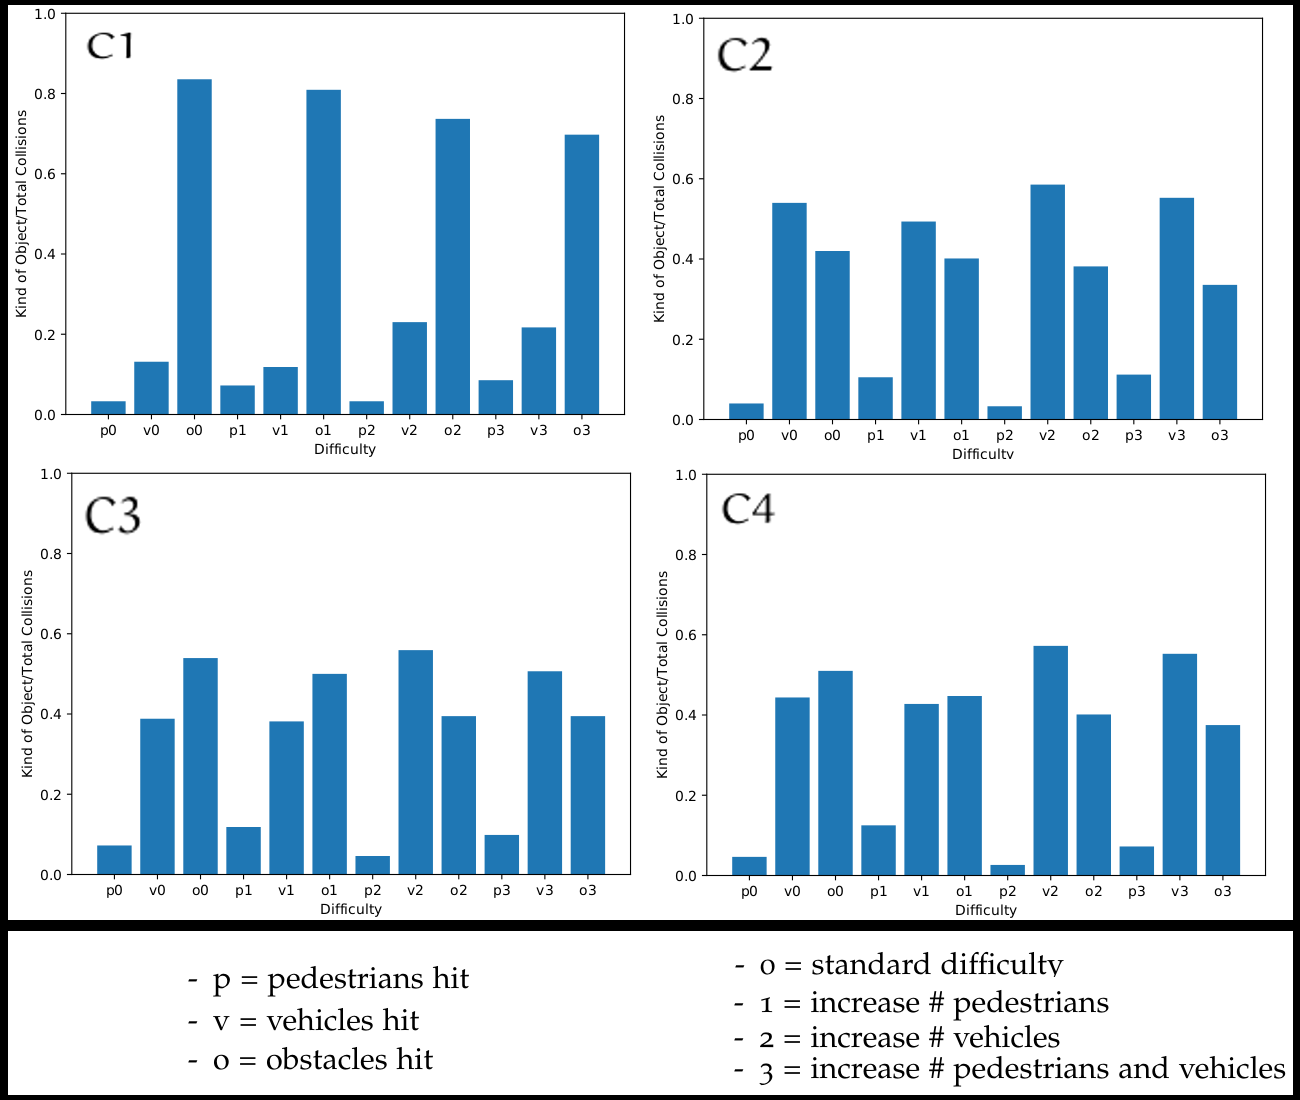
\includegraphics[width=\textwidth]{img/hit-ratios.png}
	\caption{Charts that shows $\frac{\# \: kind\: hit}{Total\: Collisions}$ for Checkpoints $1\dots 4$, in each difficulty level}
\end{figure}

These diagrams are useful to have an overlook of how the System performs when changing the difficulty of the Scenario while being trained and to observe correlations between the kinds of collision and the Checkpoints.
As we could expect, the first Checkpoint mostly collides with off-road obstacles, indicating poor driving skills of the Controller.

It also seems that there is a tendency in which the ratio of collisions with generic obstacles follows the overall Checkpoint's performances.
Observing this diagram and those of the Reliability Function, it can be seen that C1 (lowest MTTF), tends to crash against obstacles, C2, which had the best performances in terms of MTTF and MDTF, has the lowest ratio of collisions against obstacles. C3 increased the rates of these collisions, coeherently with its worsening of the MTTF/MDTF, which is subsequently lowered by C4.\newline

The four levels of difficulty defined, even if quite simple, proved to be a good way to assess the System's performances in environments that are different from the training environment. MTTFs and MDTFs are sensibly lower in difficulties 3 and 4 (increasing the number of vehicles, increasing the number of pedestrians and vehicles) giving evidences that situations of dense traffic tend to be harder to handle. At the same time increase/decrease of the hit rates with a specific kind of object, follows the features of the difficulty chosen. This suggests that the crashes observed are strictly dependent on the environmental conditions. Increasing the number of pedestrians resulted in more collisions with these \textsl{"objects"} and increasing the number of vehicles shows the same evidence. Increasing the amount of pedestrians and vehicles shows that collisions with other cars is still the main cause of a crash, giving evidences that dense traffic is more likely to create harder situations for the Controller.

These aspects are useful for the definition of more complex difficulties. These measures also allows to detect correlations between the increase/decrease of kind of collisions.\newline

With the methodology defined for the first phase, combining the definition of the Scenarios, the difficulty levels and the metrics chosen, allows to observe many features of the Controller without actively observing its executions. Moreover, combining the few metrics chosen it is possible to have an overlook of possible correlations between environmental conditions, initial conditions, and Checkpoints.


\subsection{Phase 2 - Monitor Testing}

After the Controller has been tested, and its runs are recorded, it's possible to test the Safety-Monitor in order to approximate its prediction accuracy, but also how it affects the safety of the whole System.

As said before, LiDAR data are collected at each frame and sent to the Safety-Monitor. These data are then processed using the algorithm described in the \textsl{Monitor Implementation} section and a message is sent back to the Control System, containing informations about whether braking or not. There is no synchronization between these 2 components, as it is in real systems of this kind: it would not be possible for the Controller to wait for the message of the Safety-Monitor at each frame, as it would result in jerky runs.

The \textsl{amounts} of True Positives, True Negatives, False Positives and False Negatives are computed using the procedure described in the previous chapter\footnote{We know that \textsl{rates} for these measures are linked to each other, but some of the aggregated measures (e.g.  \textsl{Accuracy}) explicitly requires \textsl{each} of these quantities}:

\begin{itemize}
	\item The Controller runs recorded in the previous phase are repeated attaching the Safety-Monitor to the car
	\item The Safety-Monitor is allowed to generate alerts, but the safety brake is not performed until the istant of time $t$ in which the System enters in an \textsl{alert state}, defined as in Chapter 3.
	\begin{itemize}
		\item[-] The choice of $t$ is a critical parameter for the accuracy of measurements, as a choice of an \textsl{"early"} $t$ may cause a brake for an event that the Controller actually handled, and a \textsl{"late"} $t$ may result in a failure of the Safety-Monitor just because the safety brake was enabled too late. Ideally, the safety brake should be enabled as soon as there is a transition from a \textsl{safe state} to an \textsl{alert state}. Unfortunately it's not always possible (if not possible at all in complex runs) to understand when this transition happened. In this work, $t$ was approximated observing the average speed of the car wrt speed limit and the time needed to process LiDAR data and get the answer from the Safety-Monitor, and was set to 2 seconds
	\end{itemize}
	\item All the alerts generated before $t$ are considered \textsl{false positives}
	\item All the frames in which the Monitor makes a prediction \textsl{and does not} raise an alert, are considered \textsl{true negatives} 
	\item If the System managed to survive for the maximum time defined for a single run, but the Safety-Monitor raises an alert after time $t$, this alert is considered a \textsl{false positive}
	\item A successfull avoidance of the crash (if happened) because of the brake caused by the Safety-Monitor, is considered to be a \textsl{true positive}
	\item If a crash happens, regardless of whether the Safety-Monitor raised an alarm or not, it's classified as a \textsl{false negative}
	\item Once the amounts of true/false positives/negatives are known, they can be combined in more refined measures
\end{itemize}

\vspace{0.5cm}

The method developed in this work seems a promising mean not only to observe the Monitor's behaviour, but also to understand and validate the hypothesis on the Controller's behaviour.\newline

Analyzing table 1, it seems like the Monitor's effectiveness is influenced by the Controller's reliability. If on one hand the True Positive Rate is stable around $0.75$ (except for $C2$, which anyway exhibited a weird behaviour in its runs), on the other hand we can see how the \textsl{Precision} of the Monitor drops after $C2$ (recall that \textsl{Precision} in this setting measures the rate of crash avoided with respect to all the alerts raised), raising some concerns on the long-term effectiveness of the Safety-Monitor. The drop in \textsl{Precision} is an indicator of the increase in \textsl{false positives} (i.e. false alarms), which makes us wonder on the fact that the Monitor is not able to classify the System's states correctly, due to the novel behaviour of the Controller. This hypothesis is enforced by looking at the $MCC$ of each Checkpoint, that follows the same behaviour of \textsl{Precision}, decreasing as the Controller gets trained. As the $MCC$ is a measure of the \textsl{overall} performance of the Monitor, we are interested in seeing whether it will decrease again in phase 3, after training the Controller again.

As we expected, this Monitor tends to produce many false positives (stabilizing around 1 false positive per meter). This doesn't affect the effectiveness of the monitoring methodology described, but raises some concerns on the effectiveness of a training strategy using \textsl{this} Monitor, and makes it possible to understand how the System would behave when both components (the Controller and the Safety-Monitor) works together, i.e. with a lot of "wrong" safety-brakes caused by the Safety-Monitor's false alarms.

\begin{table}[h!]
	\begin{center}
		\begin{tabular}{ |c|c|c|c|c| }
			\hline
			& C1 & C2 & C3 & C4 \\
			\hline
			TPR & 0.75 & 0.82 & 0.75 & 0.77 \\
			\hline
			FNR & 0.25 & 0.15 & 0.25 & 0.23 \\
			\hline
			FPR & 0.0029 & 0.0029 & 0.0062 & 0.0069 \\
			\hline
			TNR & 0.9971 & 0.9971 & 0.9938 & 0.9931 \\
			\hline
			ACC & 0.995 & 0.992 & 0.993 & 0.992 \\
			\hline
			PREC & 0.63 & 0.14 & 0.17 & 0.15 \\
			\hline
			MCC & 0.68 & 0.34 & 0.35 & 0.34 \\
			\hline
			FPPM & 0.52 & 1.13 & 1.02 & 1.12 \\
			\hline
		\end{tabular}
		
		\caption{Prediction Rates of the Safety-Monitor for Checkpoints 1-4}
	\end{center}
\end{table}

Observing the \textsl{Precision-Recall Plot} in figure 19 provides a quick visualization mean to observe the performance drop of the Safety-Monitor, performing well with a \textsl{"dumb"} Controller, while becoming almost disruptive with more trained Controllers.

Looking at figure 19, what surprises us about the Monitor is that, even if its performances are not good, its best performance is observed at the \textsl{hardest} difficulty, i.e. the setting where the amount of pedestrians and vehicles in the scenarios is increased. After $C1$, the second best performances are observed with the second hardest difficulty for the Controller, i.e. the setting where the amount of vehicles is increased. The correlation between what's \textsl{"hard"} for the Controller and what for the Monitor can not be treated exhaustively in this study, however, plotting these graphics showed an unexpected behaviour, motivating us to study more deeply this aspect in future works.

These data are consistent with the data collected and analyzed, as the Safety-Monitor performs well with $C1$, while almost the same performances were observed for $C2\dots 4$, with slightly better performances with $C2$.\newpage

\begin{figure}[h!]
	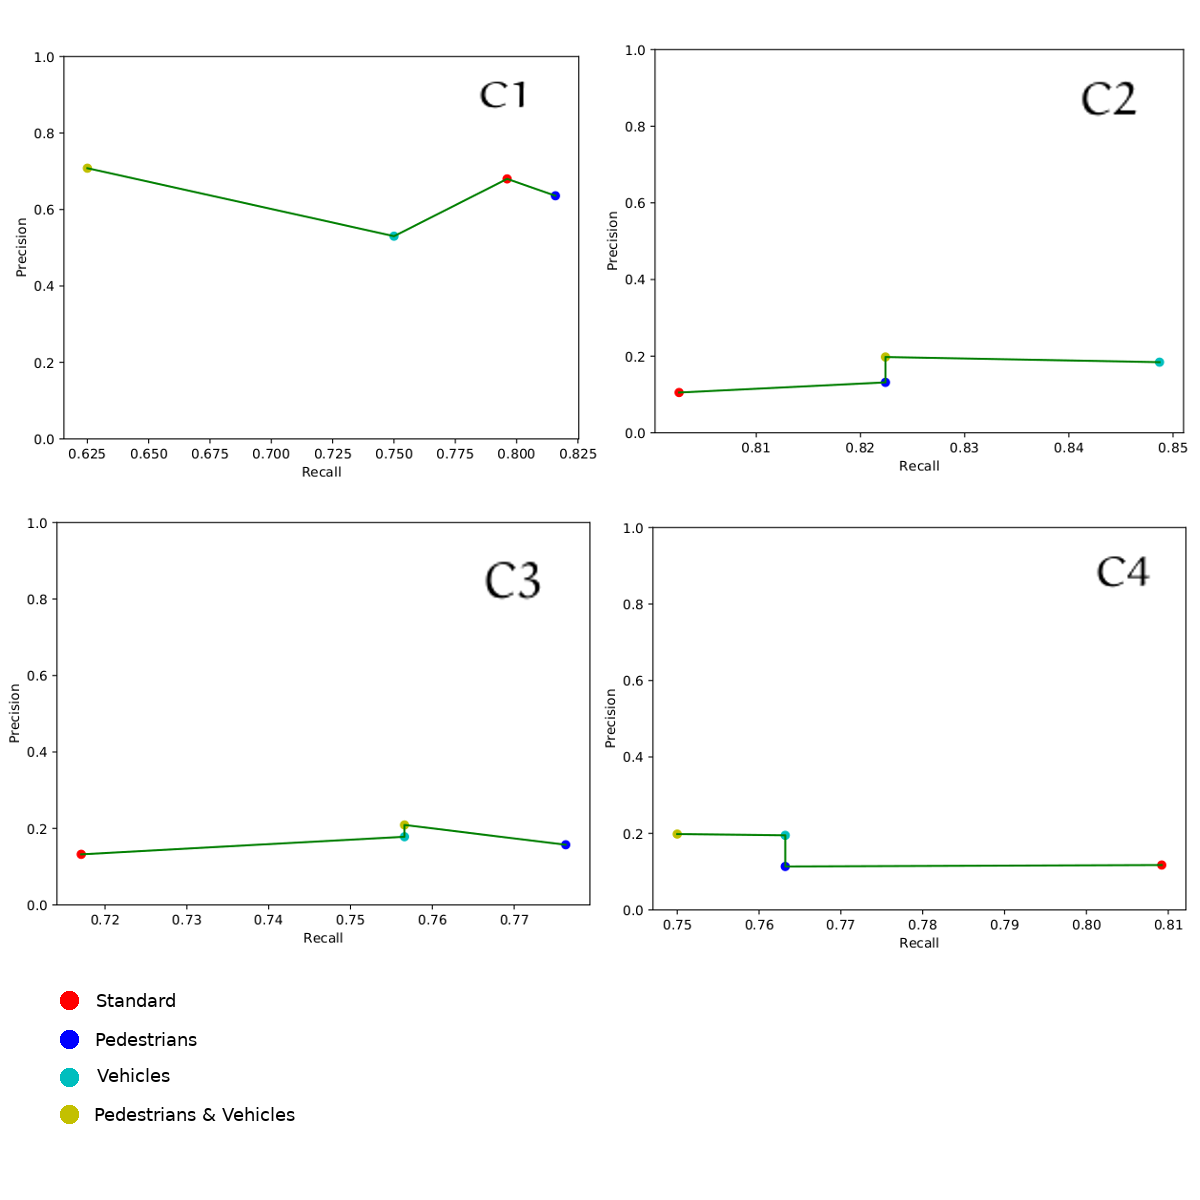
\includegraphics[width=\textwidth]{img/precision-recall.png}
	\caption{Precision-Recall Plots for Checkpoints $C1\dots 4$, using values observed in each difficulty level}
\end{figure}



In phase 1, we had to manually rerun and observe some of the best runs for Checkpoint 2, to understand the values of the Safety-Monitor's predictions. If we look at the percentage of false positives causes showed in table 3, we can see that an excessive speed is the main cause of Monitor's failures for C2.\footnote{FAST SPEED: the car's speed was over 40km/h when the crash happened.\newline SLOW SPEED: the car's speed was lower then 5 km/h when the crash happened}
Another interesting aspect that can be observed collecting data in this way, is that it seems like the more the network learns to handle new situations, the more the Safety-Monitor tends to produce more false positives and, above all, the situations that will eventually result in a crash, are of a new kind that the Monitor is not able to detect (SM ERROR).\newline
The measures listed in table 2 are just demonstrative of how this method works and how, with few measures, a lot of informations and evidences about the System's behaviour can be extracted. Depending on the actual hardware available and the simulation environment, more measures can be extracted and combined to enrich these informations.\newline

\begin{table}[h!]
	\begin{center}
		\begin{tabular}{ |c|c|c|c|c| }
			\hline
			& C1 & C2 & C3 & C4 \\
			\hline
			SM ERROR & 80\% & 41\% & 39\% & 57\% \\
			\hline
			SUDDEN STEER & 0\% & 9\% & 24\% & 12\% \\
			\hline
			FAST SPEED & 19\% & 48\% & 36\% & 30\% \\
			\hline
			SLOW SPEED & 1\% & 2\% & 1\% & 1\% \\
			\hline
		\end{tabular}

	\caption{Percentage of \textsl{false negatives} causes for $C1\dots C4$.}
	\end{center}
\end{table}

As we hypothesized at the beginning of this work, the Monitor effectiveness seems to be influenced by \textsl{how} the Controller behaves. Most importantly, data suggests that the prediction accuracy of the Monitor is not directly dependent on how long the Controller is trained. Retraining the Network again with different strategies and apply the same monitoring method for the Controllers thus obtained may confirm or deny this fact.




\subsection{Phase 3 - Retraining and Retesting}

If \textsl{phase 2} already gave some hints about the fact that the effectiveness of the \textsl{same} Safety-Monitor is likely to change when applied to different Checkpoints, the re-training with different strategies and the performance comparison of the Controllers trained with such strategies and the one we took as the default strategy, will be central in confirming or denying this hypothesis.

In this phase, we took $C4$, and trained it again using these five strategies:

\begin{itemize}
	\item[S0)] The default strategy provided by \textsl{Coach framework} and that was used to train $C1\dots 4$, where the reward function computed based on the overall neural network performances (collisions, time spent off-road or off-lane, travel speed\dots)
	\item[S1)] The reward function is now more punitive when the car hits something, while braking is slightly more rewarded, provided that the Car won't stop moving
	\item[S2)] The Safety Monitor is attached to the system and, if an alert is raised, the action of the network is replaced by the Monitor's action (the safety-brake)
	\item[S3)] The network's action is replaced by the monitor's if it raises an alert. The network is given a positive reward for behaving like the Monitor
	\item[S4)] The training step is stopped and the network is given a \textsl{negative} reward if an alert is raised
\end{itemize}

resulting in $\{C5_{S0},\: C5_{S1},\: C5_{S2},\: C5_{S3},\: C5_{S4}\}$.



\subsubsection{- On the Failure of Strategies S2, S3, S4:}

Unfortunately, the strategies that used the Safety-Monitor did not give the results we expected. Specifically, S3 and S4 turned to make the Controller to not move, while S2 makes the Controller stop after very few meters travelled if there is an object in front of the car, even if very far. All these Checkpoints doesn't get an unintentionally high reward for their behaviour, as \textsl{not moving} is given a negative reward, hence the case in which the neural network got stuck in a \textsl{local minimum} may still be an hypothesis, but our conjecture is that the training activity was too short.

This is almost surely caused by the very high false positives of the Monitor. A long training conducted in this way taught the car to not move in order to avoid the alerts raised by the Safety-Monitor and, even if these strategies takes into account the eventuality in which the Car does not move, punishing it with a negative reward, this was not enough to prevent the car from standing still.
We believe that the \textsl{reward functions} for the \textsl{DDPG algorithm} used for the training activity are well specified, in the sense that all the positive and negative behaviours were taken into account when designing it and istantaneous rewards are designed to be well-balanced, as there are no \textsl{unintentional high reward}. However, the complexity and multitude of situations that a network must be able to handle in order to drive a car, makes it very difficult to tune all the reward parameters in order to prevent outcomes like the one we had. Most of all, we can not be sure whether this behaviour is a result of \textsl{how} the reward function was designed or if a \textsl{longer} training was needed to observe interesting behaviours.

The biggest issue in the training activity is the extreme time consumption, and it's not thinkable to train $n$ agents with $n$ strategies and wait for them to be trained to analyze which strategy gave the best result.

As shown in several works, the tuning of the network's parameters largely depends on \textsl{rules-of-thumb} and \textsl{heuristic techniques}. However, these approaches has proven to be time-consuming (trial-and-error) and \textsl{error prone} (heuristics can not always model efficiently the complexity of these systems).
Moreover, at the current state of knowledge, trial-and-error seems like the only way to assess the goodness of the reward function. This problem, which is specific to these kind of algorithms, is still unsolved since \textsl{reinforcement learning} is still being studied, and there are no official regulations for self-driving cars. \cite{rewardtrialanderror2}

The design of the \textsl{reward function} for these relatively new algorithms is a hot topic in the academic community, and researchers are working on methods that aims at understanding \textsl{how} to specifiy a \textsl{good model} for the learning agent. \cite{reward1} \cite{reward2} \cite{reward3}

At the same time, as said before, AVs training require lots of data that are often unavailable or insufficient than those of conventional training techniques. There are several proposals on frameworks to be used to guide the design of decision-making policies for reinforcement learning, however most of them seems to \textsl{speedup} the learning process rather than helping on how to introduce new learning parameters for these networks. \cite{rewardtrialanderror1}

An interesting approach would be to develop stochastic models to guide us in the tuning of the reward function parameters, in order to perform a \textsl{calibration activity} prior to the retraining phase of the Controller. In this sense, the method developed in this work would be have a strong impact on the development of these models, as the performance measures for the Safety-Monitor were approximated effectively (e.g. the high false positives rate of the Safety-Monitor was a concern for us when training the Controller with the Monitor).\newline

In general, it's not clear \textsl{a priori} what value the reward function should assign to each state. We also must consider that we are working in a \textsl{continuous space state}, which is hard to model and makes hard to consider all the possible events and transitions that may happen, making this task even harder.

Unfortunately, the complexity and the novelty of these systems and techniques, still requires more research to solve these problems, and the development of a \textsl{stochastical model} to guide us in the parameter tuning will be of uttermost interest in future works.


\subsubsection{- Performance Comparison and Analyis of S0 and S1:}

The failure of the strategies that relied on the Monitor, doesn't allow us to analyze how the effectiveness of the Monitor is influenced by those strategies. However, the monitoring activity can still be performed on $C5_{S0}$ and $C5_{S1}$ to observe:

\begin{itemize}
	\item[a)] How the effectiveness of the same Safety-Monitor is influenced by the Controller's effectiveness
	\item[b)] If harshening the punishments (negative rewards) during the training has an impact on both the Controller's and Monitor's performances
\end{itemize}

The monitoring activity is basically a repetition of \textsl{phase 1} and \textsl{phase 2}. The same measures are computed and aggregated in the same form for the purpose of comparison.

$C5_{S1}$ performed significantly better than $C5_{S0}$ both in terms of MTTF and MDTF and both of them outclassed $C1\dots 4$. This reassure us on the fact that the System is actually travelling and higher MTTF is not a result of the car not moving, as happened for $C5_{S2\dots 4}$.

This is an interesting result, from the moment that the training period was the same for both Controllers (someone could argue that $C5_{S1}$ was trained for more time, but this is not the case), a more punitive strategy applied after a certain training phase gave good results in terms of running times and travelled distances, as shown in figures 20-21 which plots the Reliability Functions of $C5_{S0}$ and $C5_{S1}$ related to operational time and travelled distance.

\vspace{0.5cm}

\begin{figure}[h!]
	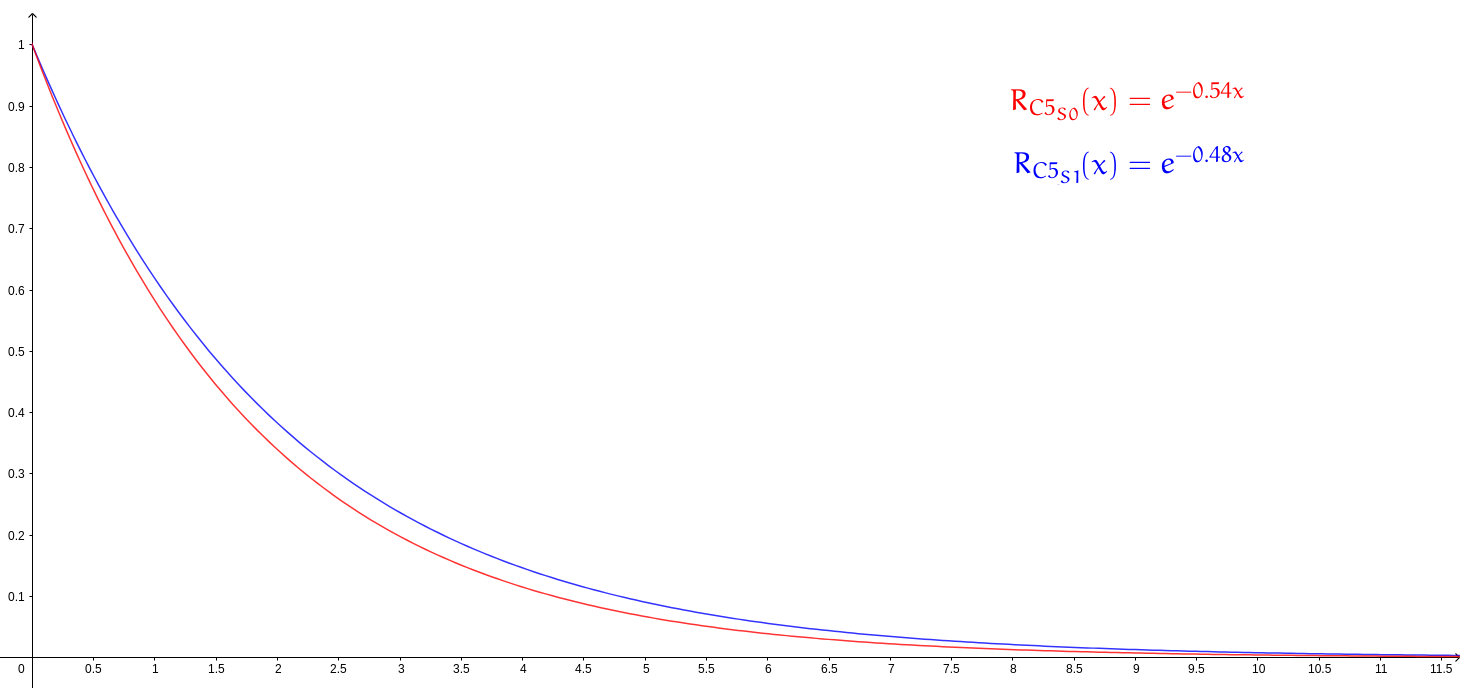
\includegraphics[width=\textwidth, height=9cm]{img/reliability-pro-stupid-comparison.png}
	\caption{Reliability Function (minutes of operation) comparison between $C5_{S0}$ and $C5_{S1}$}
\end{figure}

\begin{minipage}[c]{\textwidth}
	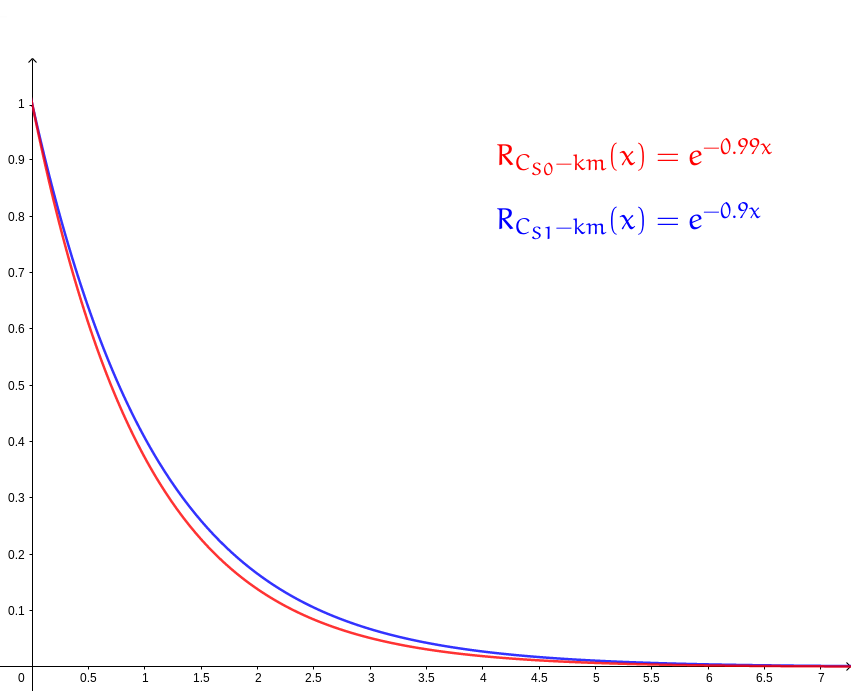
\includegraphics[width=\textwidth]{img/reliability-pro-stupid-km-comparison.png}
	\captionof{figure}{Reliability Function (kilometers travelled) comparison between $C5_{S0}$ and $C5_{S1}$}
\end{minipage}

\vspace{0.8cm}


Comparing travelled distances charts (figures 22-27), we can see that both $C5_{S0}$ and $C5_{S1}$ have good performances compared to $C1\dots 4$, as both of them have an average distance travelled of circa 1 km, while $C4$ did approximately 500 m. $C5_{S1}$ reached the max run legth 3 times, and in general did longer runs than $C5_{S0}$ which reached max length only once.
This is validated by the Reliability Functions computed both in term of time in operation and distance travelled, as $R_{C5_{S1}} > R_{C5_{S0}} > R_{C4}$.

Looking at $C5_{S1}$, if on one hand it had the best overall performances in terms of MTTF/MDTF, there are many scenarios in which it fails earlier than $C4$, failing even before the lower bound of $22$ seconds previously observed. This can be seen very clearly looking at the right side of charts (approximately after scenario 120), where if on one hand $C5_{S0}$ is learning how to handle some of those scenario (while of course still failing in others, as it would have required too much time to wait for it to master all of them), $C5_{S1}$ shows a total different behaviour and in general it performs worse than both $C4$ and $C5_{S0}$ in those scenarios.


\begin{minipage}[c]{\textwidth}
	\includegraphics[width=\textwidth]{simulations/genstupid/standard/distance-travelled-figure.pdf}
	\captionof{figure}{Meters travelled by $C5_{S0}$ in each scenario at standard difficulty}
	\vspace{0.5cm}
	\includegraphics[width=\textwidth]{simulations/genpro/standard/distance-travelled-figure.pdf}
	\captionof{figure}{Meters travelled by $C5_{S1}$ in each scenario at standard difficulty}
\end{minipage}

\begin{minipage}[c]{\textwidth}
	\includegraphics[width=\textwidth]{simulations/gen4/standard/distance-travelled-figure.pdf}
	\captionof{figure}{Meters travelled by $C4$ in each scenario at standard difficulty}
	\vspace{0.5cm}
	\includegraphics[width=\textwidth]{simulations/genstupid/standard/distance-travelled-figure.pdf}
	\captionof{figure}{Meters travelled by $C5_{S0}$ in each scenario at standard difficulty}
\end{minipage}

\begin{minipage}[c]{\textwidth}
	\includegraphics[width=\textwidth]{simulations/gen4/standard/distance-travelled-figure.pdf}
	\captionof{figure}{Meters travelled by $C4$ in each scenario at standard difficulty}
	\vspace{0.5cm}
	\includegraphics[width=\textwidth]{simulations/genpro/standard/distance-travelled-figure.pdf}
	\captionof{figure}{Meters travelled by $C5_{S1}$ in each scenario at standard difficulty}
\end{minipage}


To have a better understanding on how these Controllers behaves, we look at how many times they reached a goal in each difficulty level (figure 28), and combine this information with \textsl{MTTFs} and \textsl{MDTFs}.

What confirms our hypothesis on $C2$'s performances is that it reaches few goals compared to the others. This validate the hypothesis that the longer \textsl{MTTFs} and \textsl{MDTFs} were a result of \textsl{"lucky"} runs.

\vspace{1cm}

\begin{minipage}[c]{450px}
	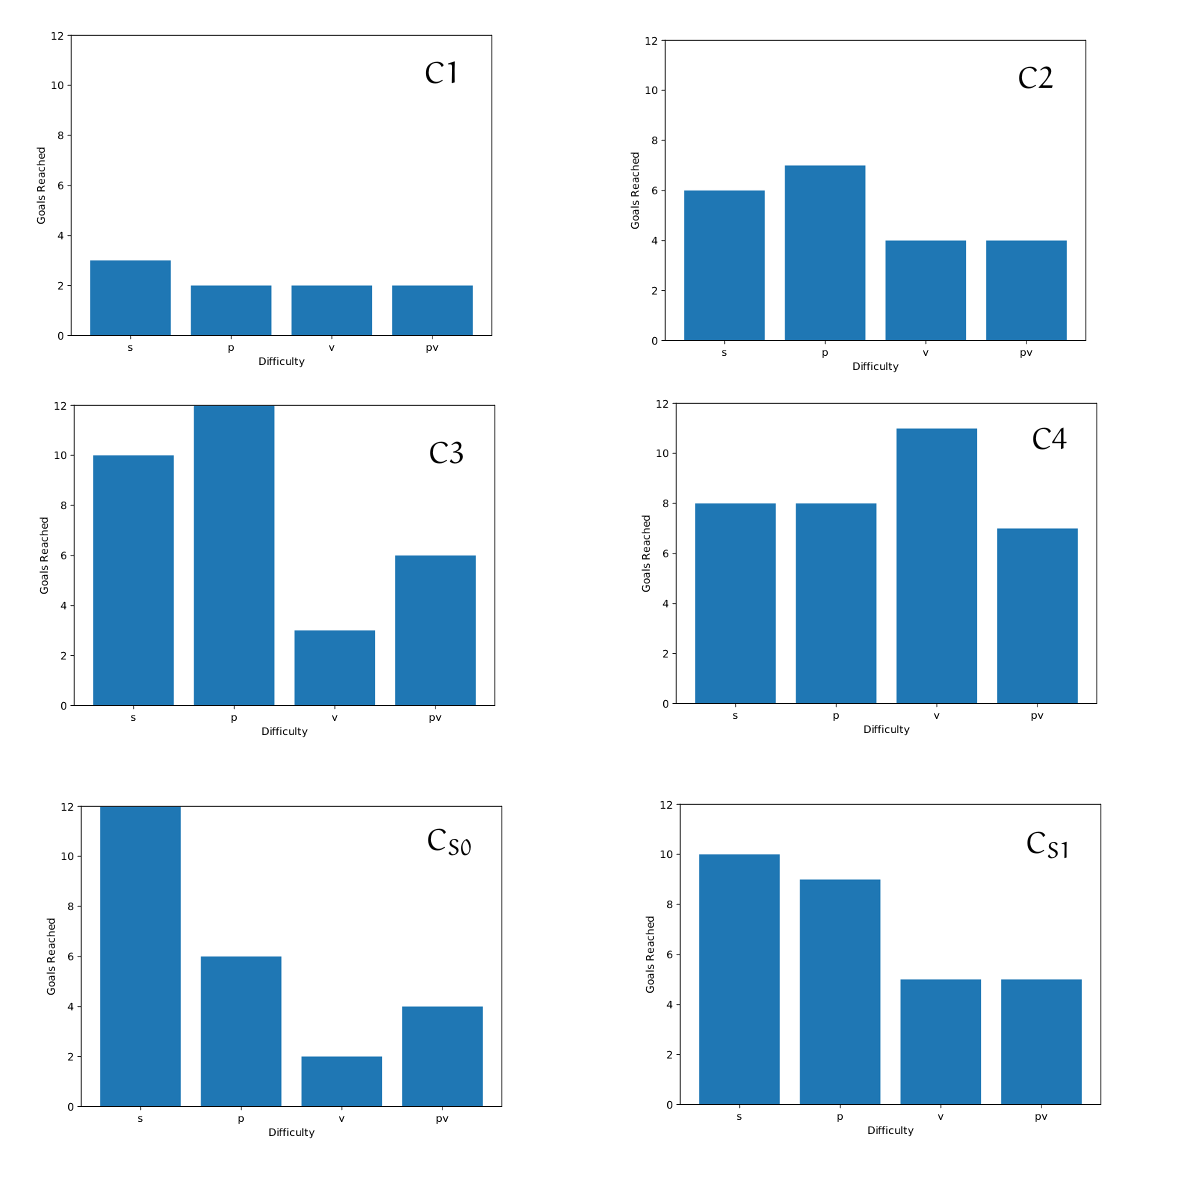
\includegraphics[width=450px,height=450px]{img/goals.png}
	\captionof{figure}{Goals reached charts for each Checkpoint, in each difficulty level}
\end{minipage}
\newpage

Moreover, $C5_{S1}$ chart is more balanced in terms of goals reached per difficulty. A fair objection would be that $C4$ reached its goals more times, but the average distance travelled is significantly lower than both $C5_{S0}$ and $C5_{S1}$, moreover, as an indicator of the fact that $C4$ \textbf{is not} better than $C5_{S0}\: \&\: C5_{S1}$, by an analysis of raw data it was observed that:

\begin{itemize}
	\item $C5_{S1}$ is capable of reaching \textsl{more} goals in the \textsl{same} run, differently from the other Checkpoints
	\item $C4$ reaches some goals in scenarios $> 120$, where the unexpected performance drop is observed for $C5_{S1}$
\end{itemize}

In addition to this, $C5_{S0}$, which is the \textsl{"natural continuation"} of $C4$ as it is obtained from $C4$ using the \textsl{same} training strategy, performs very good at \textsl{standard difficulty} while performing much worse in the others, fact validated by comparing times to failure in each difficulty as $MTTF_{C5_{S0}h_{0}} >> MTTF_{C5_{S0}h_{1\dots 3\dots 3}}$.
This seems to suggest that the training strategy adopted has a strong influence on how the System will perform in conditions different from the training ones. Collected data confirm this, as looking at raw data, we observe that $MTTF_{C5_{S1}h_{i}} > MTTF_{C5_{S0}h_{i}}$ as a proof that $C5_{S1}$ performs better in harder conditions. Moreover, the differences observe on the average travelled distances are lower than the ones observed for \textsl{all} the other Controllers, which again reassure us on this fact.\newline

As done for $C1\dots 4$, hit rates of collisions with specific kinds of object wrt to total collisions are computed and shown in figure 29. Those for $C5_{S0}$ and $C5_{S1}$ looks similar, as hit rates take close values. The drop of collision rate against \textsl{obstacles} reassure us on the fact that both Checkpoints are now learning to stay on-road. To confirm this fact, a subset of runs was analyzed and it was observed that the main cause of collisions with generic obstacles is caused by the Car actually trying to avoid other cars and pedestrians. The same phenomenon was observed for Checkpoints $C3,\: C4$, where huge increasement of obstacles hit was linked to an increase of SUDDEN STEER errors for the Monitor.
More evidences about this fact will be probably given by analyzing the runs with the Safety-Monitor attached to the System.


\begin{minipage}[c]{\textwidth}
	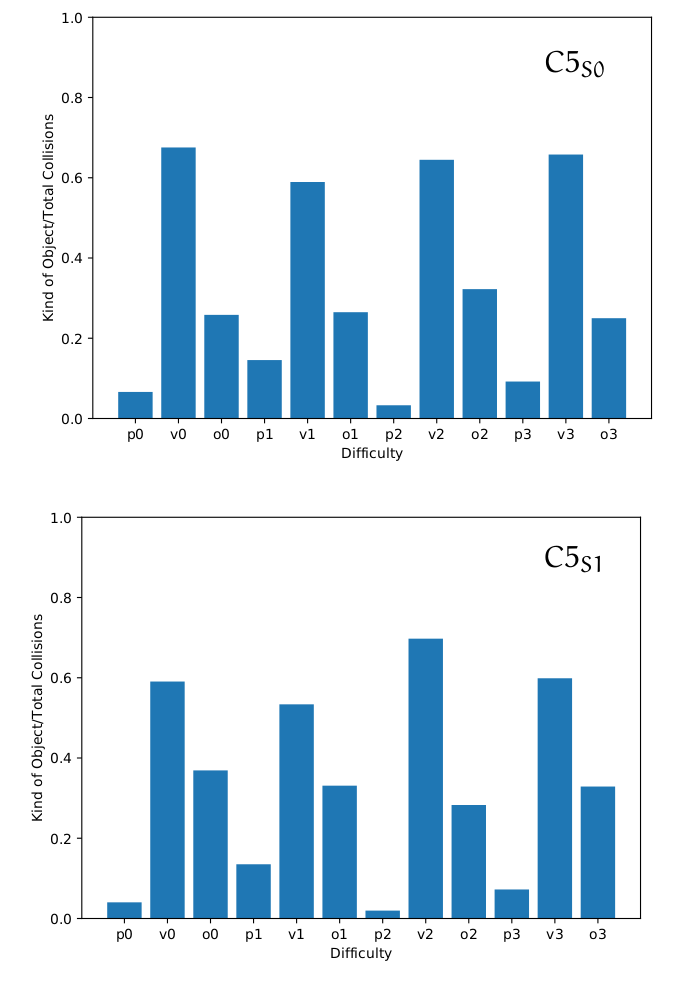
\includegraphics[width=\textwidth]{img/hit-ratios-stupid-pro.png}
	\captionof{figure}{Hit rates for $C5_{S0}$ and $C5_{S1}$}
\end{minipage}

\subsubsection{- On the Effectiveness of the Safety-Monitor:}

The analysis of the Safety-Monitor performances isn't different from what we did in \textsl{Phase 2}.

This second assessment of the Safety-Monitor seemed promising in conferming the fact that the effectiveness of the Safety-Monitor strongly depends both on the \textsl{training strategy} adopted and on the Controller's performances.

Looking at tables 4 and 5, we can see that the Monitor attached to $C_{1\dots 4}$ and $C5_{S0}$ have a \textsl{True Positive Rate} of approximately $0.75$, with the exception of $C2$, that acted as an outlier in our study. The fact that the Monitor with $C5_{S0}$ has the same TPR of the previous Checkpoints is a good result, and a promising starting point for further examinations. However, to claim this fact, more data and analysis are needed and will be a central point in our next studies.\newline

\begin{table}[h]
	\begin{center}
		\begin{tabular}{ |c|c|c| }
			\hline
			& $C5_{S0}$ & $C5_{S1}$ \\
			\hline
			TPR & 0.74 & 0.67 \\
			\hline
			FNR & 0.26 & 0.33 \\
			\hline
			FPR & 0.0058 & 0.0059 \\
			\hline
			TNR & 0.9942 & 0.9941 \\
			\hline
			ACC & 0.994 & 0.994 \\
			\hline
			PREC & 0.10 & 0.09 \\
			\hline
			MCC & 0.28 & 0.25 \\
			\hline
			FPPM & 0.99 & 0.89 \\
			\hline
		\end{tabular}
		\caption{Prediction Rates of the Safety-Monitor for Checkpoints $C5_{S0},\: C5_{S1}$}
	\end{center}
\end{table}

\begin{table}[h]
	\begin{center}
		\begin{tabular}{ |c|c|c|c|c||c|c| }
			\hline
			& $C1$ & $C2$ & $C3$ & $C4$ & $C5_{S0}$ & $C5_{S1}$ \\
			\hline
			TPR & 0.75 & 0.82 & 0.75 & 0.77 & 0.74 & 0.67 \\
			\hline
			FPR & 0.0029 & 0.0029 & 0.0062 & 0.0069 & 0.0058 & 0.0059 \\
			\hline
			FPPM & 0.52 & 1.13 & 1.02 & 1.12 & 0.99 & 0.89 \\
			\hline
			ACC & 0.995 & 0.992 & 0.993 & 0.992 & 0.994 & 0.994\\
			\hline
			PREC & 0.63 & 0.14 & 0.17 & 0.15 & 0.10 & 0.09\\
			\hline
			MCC & 0.68 & 0.34 & 0.35 & 0.34 & 0.28 & 0.25 \\
			\hline
		\end{tabular}
		
		\caption{Main measures comparison for every Checkpoint}
	\end{center}
\end{table}

As a proof that true and false positive and negative rates were not enough to understand the Monitor's performances, we can again look at the values of \textsl{Precision} and \textsl{MCC}. Analyzing these measures, the decrease in both of them immediately catches the eye. If Precision decrease relatively slowly, the drop in $MCC$ is considerable, passing from $\approx 0.35$ observed in $C2,\: C3,\: C4$ to $0.28$ and $0.25$ observed in $C5_{S0}$ and $C5_{S1}$ respectively. The decrease in the $MCC$ worries us, as this monotonic decrease could make the $MCC$ to become negative (i.e. actually \textsl{detrimental} to the System, making wrong predictions only), if the Controller gets trained again.

The most interesting fact is that the Monitor performed worse with $C5_{S1}$ which is actually the Controller that had the best performances in terms of MTTF/MDTF. The fact that this last Checkpoint was obtained from $C4$ by \textsl{changing} the training strategy, seems to motivate our initial hypothesis both on the long-term effectiveness of the Safety-Monitor, and the influence the training strategy has on it. 
Another interesting fact is the drop in TPR.

We observe again the \textsl{Precision-Recall Plots} for the Safety-Monitor attached to $C5_{S0}$ and $C5_{S1}$, and we can see that the Monitor is definetely useless and almost disruptive to the System. From these plots, the Monitor worsening when operating with $C5_{S1}$ can be immediately seen, as it ranges from $0.65$ to $0.685$, while with $C5_{S0}$ it ranges from $0.7$ to $0.8$, consistently with $C1\dots 4$. Moreover, these plots confirm that, even if its performances are still bad, that the Monitor has overall better performance with difficulties $h2,\: h3$, the two hardest difficulties defined, as it was observed with the previous Checkpoints.

\begin{minipage}[c]{\textwidth}
	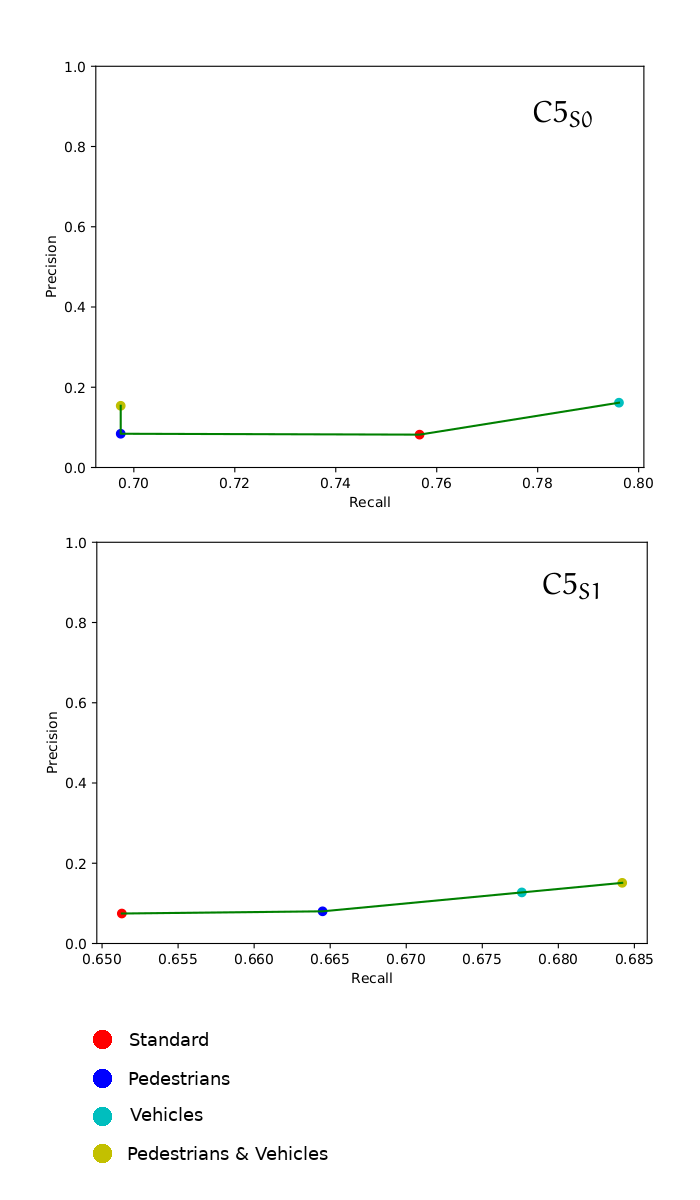
\includegraphics[width=\textwidth]{img/precision-recall-prostupid.png}
	\captionof{figure}{Precision-Recall Plot for Checkpoints $C1\dots 4$, using values observed in each difficulty level}
\end{minipage}
\newpage
\newpage


Although we could not plot the ROC curve, for the reasons explained in Chapter 3, the \textsl{Precision-Recall Plot} proved to be an effective visualization mean for this kind of systems, where there is a huge imbalancement between the positive and negative classes. The performance drop of $C5_{S1}$ would have not been that immediate with the "classic" ROC curve, as the False Positive Rates all have values lower than $10^{-2}$, resulting in curves flattened to the left side of the plot. Moreover, due to this issue, it would have been harder to understand how the Monitor performs in each difficulty.
Ddespite the missing ROC plot, with our methodology we were still able to correctly define and measure all the rates needed to evaluate a classification model. What surprises us, looking once again at table 5, are the TPR and FPR values observed for $C5_{S0}$ and $C5_{S1}$: even if the Monitor had close FPR values with both of them, the drop in TPR observed in $C5_{S1}$ seems like a speedup towards the "worse-than-random area" (enforced by the $MCC$ decreasing monotonically), motivating the fact that the Controller is now creating more situations that the Monitor is not able to detect (also motivated by the fact that it $C5{S1}$ shows the lowest FPPM ever, excluding $C1$).
It is true that a deviation from the mean value is observed with $C2$ as well, but the other measures were somehow consistent and got close values. $C5_{S0}$ has the same TPR of all $C1\dots 4$ and it was trained with the same strategy of $C1\dots 4$. This doesn't happen with $C5_{S1}$, but at the same time, we can not claim this as a fact, as more experiments are needed. Again, this result may be a starting point for future works.\newline

Analyzing crash causes listed in table 6, we have another interesting result. The percentage of \textsl{"unknown"} causes, labeled as generic errors of the Safety-Monitor is higher for $C5_{S1}$ than $C5_{S0}$, which is the main cause of crashes for the first, while the latter tends to crash at high speed. This may ring a bell on the fact that $C5_{S1}$, which now we can confirm performed better than \textsl{all} the other Checkpoints, gets into situations which are more complex to handle. This is a very important point to analyze. A fair objection would be that our Safety-Monitor is not good enough to detect the new kinds of hazard caused by the novel Controller's behaviour. It is true that a more sophisticated Monitor would be able to detect and avoid more complex hazardous events, and it may even show a SM-ERROR rate of $0\%$ when tested with a controller $C_{i}$, but what we are pointing out in this work is that \textsl{we can not assure} that if $C_{i}$ is trained to drive in \textsl{new environments}, obtaining $C_{i+j}$, the SM-ERROR rate will still be $0\%$.

The high percentage of FAST SPEED errors observed in $C5_{S0}$ also provides a deeper explanation on the higher collision rate against pedestrians and vehicles: in many scenarios the System is goind so fast that it is not able to detect the possible pedestrians/vehicles on its road. At the same time, the similarity in the observed hit rates assure us that both Checkpoints are learning to don't go off-road and raises more questions on \textsl{how} the definition of the reward function causes behaviours that were not specifically planned or considered, when designing the training strategy.

\begin{table}
	\begin{center}
		\begin{tabular}{ |c|c|c| }
			\hline
			& $C5_{S0}$ & $C5_{S1}$ \\
			\hline
			SM ERROR & 28\% & 50\% \\
			\hline
			SUDDEN STEER & 14\% & 13\% \\
			\hline
			FAST SPEED & 58\% & 37\% \\
			\hline
			SLOW SPEED & 0\% & 0\% \\
			\hline
		\end{tabular}
		\caption{Percentage of \textsl{false negatives} causes for $C5_{S0},\: C5_{S1}$.}
	\end{center}
\end{table}